\documentclass[journal,10pt,onecolumn,compsoc,letterpaper,draftclsnofoot,table,xcdraw]{IEEEtran} \usepackage[margin=0.75in]{geometry}
\usepackage{pdfpages}
\usepackage{minted}
\usepackage{graphicx,float} 
\usepackage{listings}
\usepackage{verbatim}
\usepackage{url}
\usepackage{nameref}
\usepackage{setspace} \singlespacing
\graphicspath{/graphics} \setlength{\parskip}{\baselineskip} \setlength\parindent{24pt}
\usepackage[english]{babel}
\usepackage{fullpage}
\usepackage{hyperref}
\hypersetup{
    colorlinks,
    citecolor=black,
    filecolor=black,
    linkcolor=black,
    urlcolor=black
}
\title{Writing Topic 1: Processes}
\author{Behnam Saeedi\\ CS444: Operating systems II}
\date{\today}
\begin{document}
\maketitle
\begin{centering}
Spring 2017
\begin{abstract}
\noindent This document covers The implementation of processes, threads and CPU schedulers that are used in Linux, Windows and FreeBSD kernels. Initally it describes the Linux kernel and then it compares the Windows and FreeBSD kernel to Linux. Then it covers certain algorithms used in implementation. Finally it describes specific features of some of these implementations. 
\end{abstract}
\end{centering}
%--------------------------------------------------------------
\newpage
\tableofcontents
\newpage 
%--------------------------------------------------------------
% processes, threads, and CPU scheduling
\section{Linux}
\subsection{Process}
\noindent In Linux processes are instances of running programs. In linux the first process that is created with ID 1 is the init process. The processes could be viewed by two commands:
\begin{minted}{bash}
$ top
# and
$ ps
\end{minted}

\begin{figure}[h]
\centering
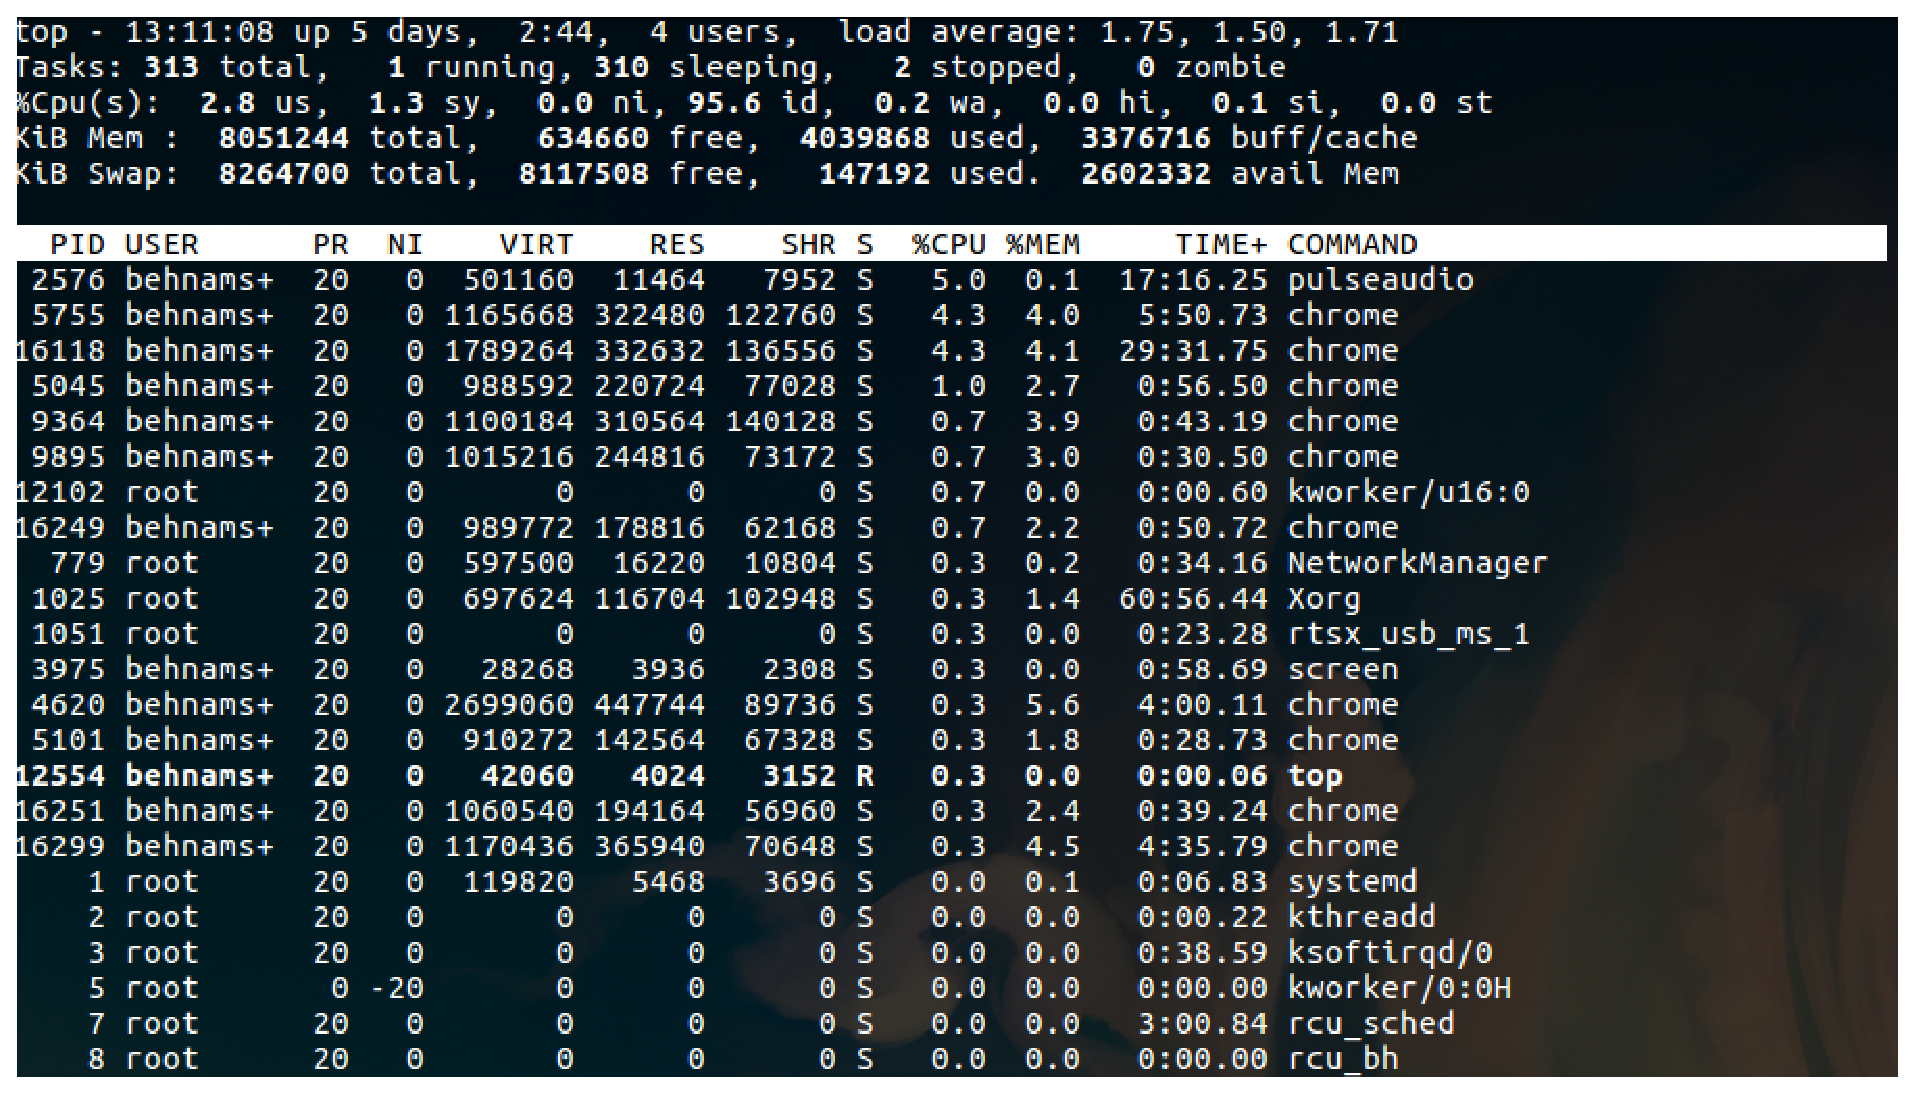
\includegraphics[width=150mm]{graphics/Top-view} \\
\caption{The view of "top" command in Linux shell}
\end{figure}

\begin{figure}[h]
\centering
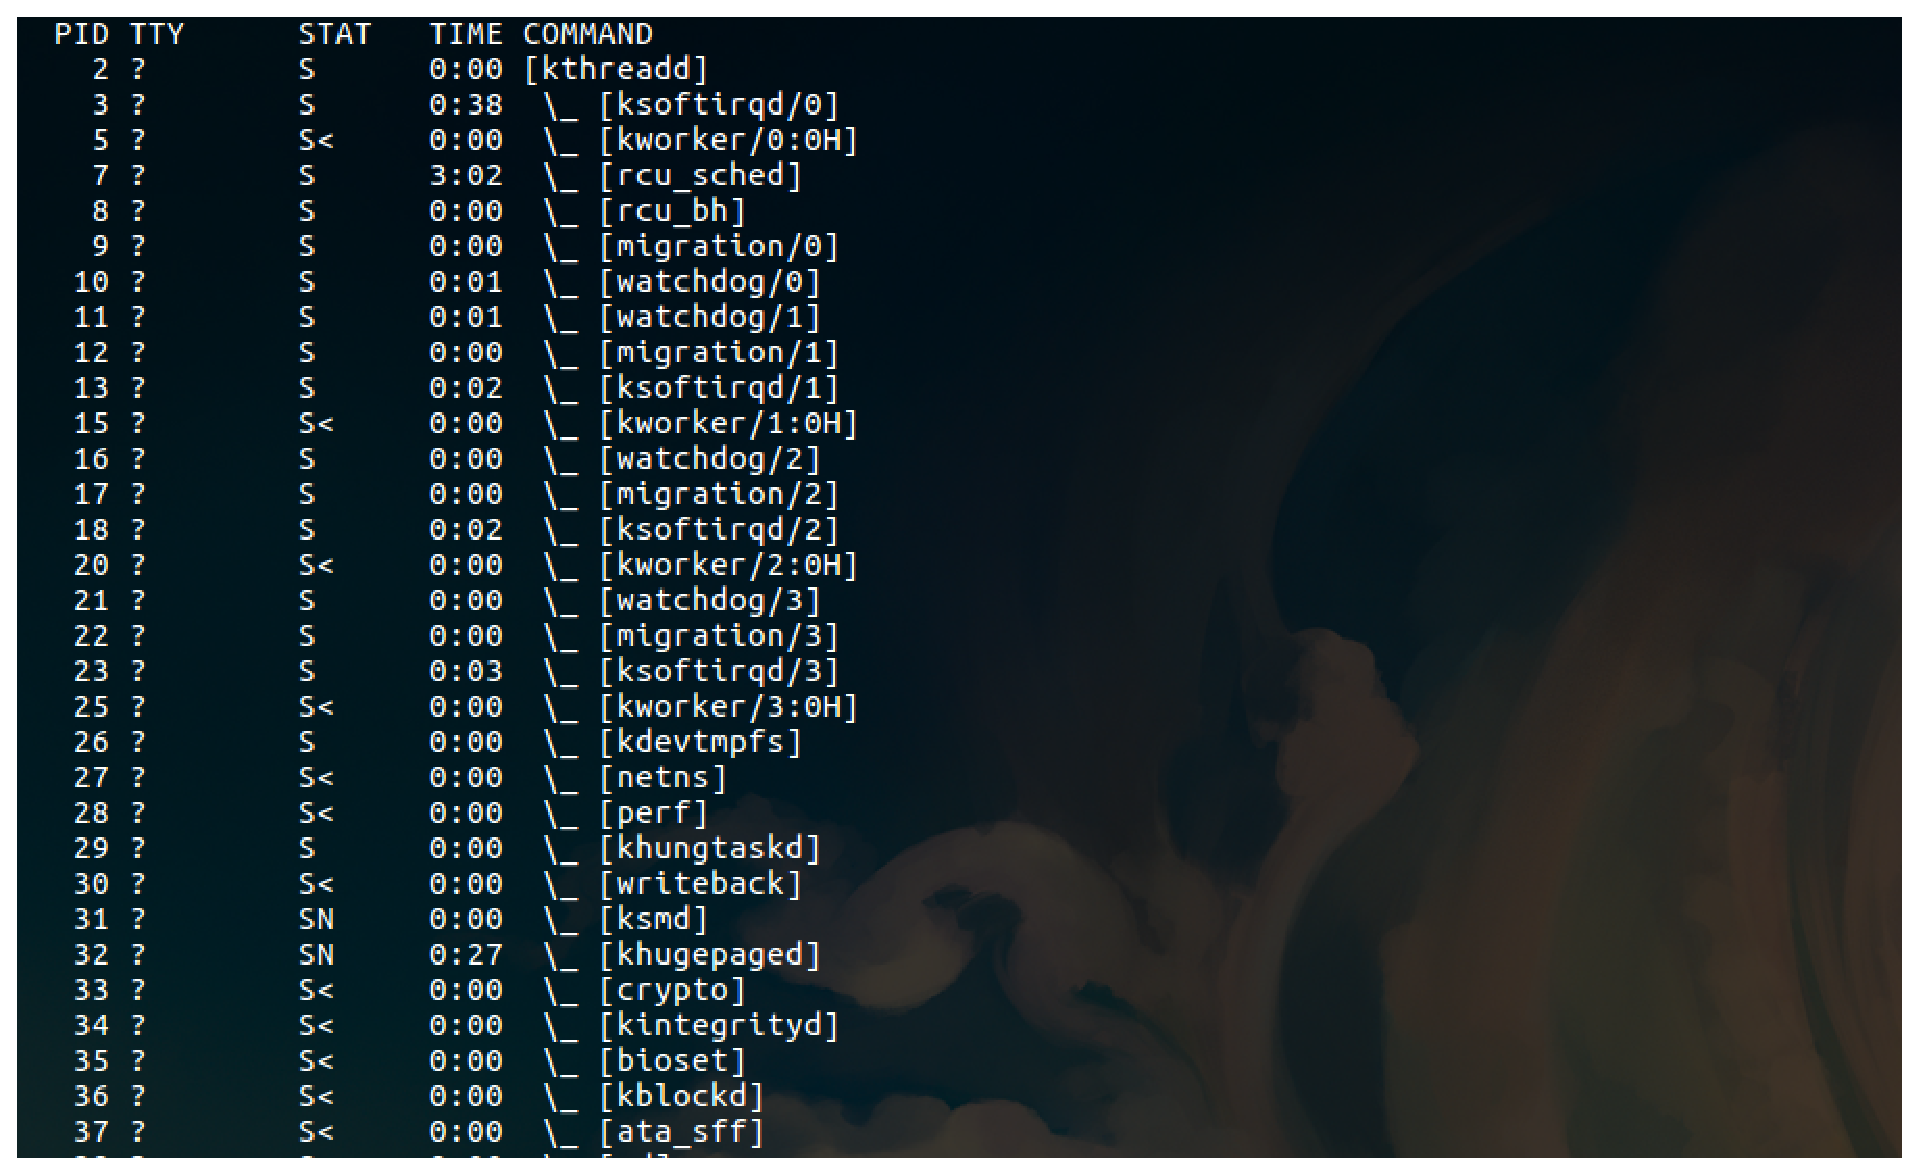
\includegraphics[width=150mm]{graphics/ps} \\
\caption{The view of "ps fax" command in shell}
\end{figure}

\noindent These two commands show a list of processes that are happening on the operating system. figures 1,2. top is a live view and ps is a static view of current processes. The init process could be found and viewed by the following command:
\begin{minted}{bash}
$ ps fax | grep [i]nit
    1 ?        Ss     0:06 /sbin/init splash
\end{minted}
\noindent Each process in Linux could be in one of the following states:
\begin{itemize}
\item \textbf{Running:} Task is being processed or is about to be assigned to CPU for process.
\item \textbf{Waiting:} interruptible and un-interruptible process waiting for resources to be assigned.
\item \textbf{Stopped:} The process has been stopped by a signal. The process is in a halt.
\item \textbf{Zombie :} This is a terminated process that is still consuming resources.
\end{itemize}

\noindent In Linux each process has an identifier and a task vectors. in order to see this feature better, Linux provides the "pstree" command:
\begin{minted}{bash}
$ pstree
systemd─┬─ModemManager─┬─{gdbus}
        │              └─{gmain}
        ├─NetworkManager─┬─dhclient
        │                ├─dnsmasq
        │                ├─{gdbus}
        │                └─{gmain}
        ├─Xvfb─┬─{llvmpipe-0}
        │      ├─{llvmpipe-1}
        │      ├─{llvmpipe-2}
        │      └─{llvmpipe-3}
        ├─accounts-daemon─┬─{gdbus}
        │                 └─{gmain}
        ├─acpid
        ├─agetty
        ├─at-spi-bus-laun─┬─dbus-daemon
        │                 ├─{dconf worker}
        │                 ├─{gdbus}
        │                 └─{gmain}
        ├─at-spi2-registr─┬─{gdbus}
        │                 └─{gmain}
        ├─avahi-daemon───avahi-daemon
        ├─bluetoothd
#			.
#			.
#			.
\end{minted}
\noindent Task vector is an array of pointers in a data structure sense that points to ever task struct data structure in the system. Furthermore, Unix introduced a system known as IPC or Inter-Process Communication. This allows different processes to communicate with one another.
%--------------------------------------------------------------
\subsection{Threads}
\noindent From the kernel's perspective there is no distinction between threads and processes. Threads are series of processes that get access to the same memory space. From a CPU and scheduling perspective each thread gets its own time slot. We can trace and see each of these threads that are related to a process. Running the following code reveals an interesting fact about the Linux processes:
\begin{minted}{bash}
$ Htop
# or
$ top -H
# or
$ ps -T -p 1
\end{minted}
\noindent init actually does not lunch any threads meaning that non of its children and the init itself would have access to the memory space of the child processes. Using the following command we can see the threads of each process:
\begin{minted}{bash}
$ ps -T -p $(ps efax | grep [m]y-app | awk '{print $1}')
# replace my-app with name of a program such as mysqld -> [m]ysqld
$ ps -T -p $(ps efax | grep [m]ysqld | awk '{print $1}')

  PID  SPID TTY          TIME CMD
 8302  8302 ?        00:00:00 mysqld
 8302  8307 ?        00:00:00 mysqld
 8302  8308 ?        00:00:03 mysqld
 8302  8309 ?        00:00:04 mysqld
 8302  8310 ?        00:00:03 mysqld
 8302  8311 ?        00:00:03 mysqld
 8302  8312 ?        00:00:03 mysqld
 8302  8313 ?        00:00:03 mysqld
 8302  8314 ?        00:00:03 mysqld
 8302  8315 ?        00:00:03 mysqld
 8302  8316 ?        00:00:03 mysqld
 8302  8317 ?        00:00:03 mysqld
 8302  8318 ?        00:00:03 mysqld
 8302  8320 ?        00:00:03 mysqld
 8302  8321 ?        00:00:05 mysqld
 8302  8322 ?        00:00:00 mysqld
 8302  8323 ?        00:00:04 mysqld
 8302  8324 ?        00:00:00 mysqld
 8302  8325 ?        00:00:00 mysqld
 8302  8326 ?        00:00:00 mysqld
 8302  8327 ?        00:00:00 mysqld
 8302  8328 ?        00:00:00 mysqld
 8302  8329 ?        00:00:00 mysqld
 8302  8330 ?        00:00:00 mysqld
 8302  8331 ?        00:00:00 mysqld
 8302  8332 ?        00:00:00 mysqld
 8302  8333 ?        00:00:00 mysqld
 8302  8336 ?        00:00:00 mysqld

\end{minted}
\noindent All of these threads use the same address space as the mysqld process that was displayed in ps. In implementation, thread is actually implemented as a process. We can imagine process as a memory space and threads as units of execution of the program. many programs have a single threads for the process. Kernel to has a 1-1 ratio between both of them, it treats threads as full processes that share the same memory space. Even we try to spawn a new thread we use the same command as spawning a new process and pass different arguments to indicate if we want our new thread to be independent process or not.
%--------------------------------------------------------------
\subsection{CPU Scheduling}
\noindent Linux uses complex data structures in order to become very efficient in binding processes to the CPU. Each processor gets its own run queue and selects processes from that specific run queue. This creates an issue where one processor ends up idling while there are processes on other processor's queue. In order to avoid this, the queues get rebalanced periodically. Each process gets a bitmask in order to identify which processor it can be processed on. This mask could be reassigned but re-balancing will not override affinity. The processor follows the following algorithm: \cite{cscedu}[page 6]
\begin{itemize}
\item Highest priority queue with runnable processes is selected
\item First process on that queue is selected
\item Quantum size is calculated
\item Runs until its time runs out
\item its put on the expire queue
\item the process repeats
\end{itemize}
\noindent As of 2007-04-13 a new patch put the CFS or completely fair scheduler in Linux kernel. \cite{cfsmemo}. As this memo mentions, a complete rewrite of the Linux task scheduler goes into place after this patch and replaces the O(1) scheduler that was used before. This scheduler follows the following algorithm: \cite{cfshw}
\begin{itemize}
\item The left most node of the scheduling tree is sent for execution.
\item If completed, it is removed from the system and scheduling tree.
\item If reached maximum execution time, it is stopped (voluntarily or via interrupt) and reinserted into the scheduling tree and a new execution time is calculated
\item repeat
\end{itemize}
%--------------------------------------------------------------
\section{Windows}
\subsection{Process}
\noindent In windows the processes are explained very similarly to Linux. A process is an executing program as described by MSDN. \cite{msdnprocess}. Windows also creates a new terminology called "Job Object". Job object allows multiple processes to be managed as a single unit. These object could have features assigned by OS such as namable, securable, etc.\cite{msdnprocess}. \\
\noindent Similarly to Linux a process gets its own independent virtual address space. Each process contains one or more independently executing threads. Threads can create threads, processes and fibers. (Fibers are explained in Fibers subsection). It appears that in Windows, Process is a container that contains all of the threads. In other words, Process describes the address space which its threads will be using. Processes could be viewed and managed using several available tools.
\subsubsection{Command: tasklist}
\noindent Windows provides few tools in order to analyze the processes. The first tool was the tasklist. It provides a list of all of the tasks and processes that are running on the processor. Later, a Graphical user interface was developed for this command with the same name.
\subsubsection{Close Program}
\noindent The second tool that was introduced was called Close Program. This gave the user the ability of controlling the programs that were running at the time. This however did not last long since by introduction of multi processing it needed to change for more versatile tools.
\subsubsection{Task Manager}
\noindent The third tool is a graphical user interface designed to display the processes that are running on the system very similarly to the top command in Linux. This GUI is the Windows Task Manager. 
%--------------------------------------------------------------
\subsection{Threads}
\noindent Threads are also similar to Linux threads. The MSDN describes the threads as the basic unit which the kernel allocates time. A thread is part of a process that actually executed the programmed code. \cite{msdnprocess}. This functionality of a process still is fairly similar to the functionality of a thread in Linux with the difference that processes do not necessarily have to have threads in Linux where in windows each process must at least have one or more threads in order to execute code. From a code perspective, Windows has a completely different sets of syntax for creation and destruction of threads and processes.\\
\noindent In order to view threads in windows there aren't any tools provided that are shipped with the kernel for the computer user. However, there are third party programs that display the threads of each process. \textbf{Process Explorer} is a third-party tool that gives the user the ability to monitor different threads in windows processes.
%--------------------------------------------------------------
\subsection{Fiber}
\noindent The MSDN document \cite{msdnprocess} introduces a concept called "fiber". Fiber is a unite of execution that is created by a thread and needs to be manually scheduled by the threads to be executed. \cite{msdnprocess}. Fibers share the thread context of their parent thread.
%--------------------------------------------------------------
\subsection{CPU Scheduling}
\noindent Windows system scheduler controls the multitasking process by deciding which processing thread will recieve the next time slice. This process takes advantage of scheduling priorities.
\subsubsection{Priorities}
\noindent There are 6 possible processing priority classes for each process.
\begin{itemize}
\item Idle
\item Bellow normal
\item Normal
\item High
\item Realtime
\end{itemize}
\noindent Each priority class itself has 7 priority levels for each thread:
\begin{itemize}
\item Idle
\item Lowest
\item Bellow normal
\item Normal
\item Above normal
\item Highest
\item Time critical
\end{itemize}
\noindent The priority classes could be managed by the user in Task Manager. By default the priority of a process is normal. The priority levels on the other hand are assigned by the developer to each thread or is inherited from the parent process. This concept is described by the nice command in Linux. \cite{windowscpuscheduling}. In windows the value of this priority is a number between 1 to 31 where 31 is the highest priority and 1 is Idle.
\subsubsection{Context Switching}
\noindent Similarly to linux the scheduler maintains a queue for ready tasks and priorities. Unlike Linux, the queue contains threads and their priorities only. The context switching happens in  5 steps:
\begin{itemize}
\item Save the context of the current thread
\item Place the current thread at the end of the priority queue
\item Find the next highest priority queue with ready threads
\item remove the new thread, load its context and execute
\item repeat
\end{itemize}
\cite{winconsw}.
\subsubsection{Algorithm}
\noindent According to last sub section, windows uses a prioritized Round-Robin technique with multi-level feedback for priority handling. This technique has been the algorithm used for scheduling since NT. However, Vista did introduce some new heuristics in order to set priorities of certain processes. This scheduler is referred to as "Multi-level feedback queue" which still is a Round-Robin scheduler. Windows has also introduced a new concept to scheduling. This concept is referred to as User-mode Scheduling or UMS.\cite{windowscpuscheduling}. This allows processes to schedule their own threads and we can see that in the fiber concept discussed earlier.
%--------------------------------------------------------------
\section{FreeBSD}
\subsection{Process}
\noindent According to the documentation of freebsd, the processes are designed very similarly to Linux processes. The commands used for monitoring them are too same as Linux.\cite{freebsdPD} 
%--------------------------------------------------------------
\subsection{Threads}
\noindent  The documentation for the freeBSD addresses 1:1 threading and 1:n Threading and describes the basics of the two threading methods. \cite{freebsdalook} Furthermore, it explains the libraries which implement threading in FreeBSD. It appears many of the features described in documentation are similar to Linux's implementation.
%--------------------------------------------------------------
\subsection{CPU Scheduling}
\noindent FreeBSD Kernel has two available schedulers. The ULE scheduler first introduced in FreeBSD 5.0 and The 4.4BSD scheduler.
\subsubsection{4.4BSD scheduler}
\noindent This scheduler was originally designed for Linux kernel in order to address interactivity issues. This scheduler has a single run-queue and is variation of Round-Robin. This queue is in fact a double linked list and is shared accross all the CPUs. The reason to that is to avoid complex load balance algorithms.\cite{freebsdpdf}[Page 2].
\subsubsection{ULE scheduler}
\noindent ULE scheduler is based on the BSD schedulerand imporves on some of its features in order to improve efficiency specially with single processor systems. This scheduler is disabled by default in favor of the traditional BSD scheduler. Furthermore, it is fair by default but it could be set to favor specific processes.
%--------------------------------------------------------------
\newpage
\bibliographystyle{IEEEtran}
\bibliography{sources}
\end{document}
